\documentclass[preview]{standalone}
\usepackage{amssymb, amsthm}
\usepackage{mathtools}
\usepackage{bm}
\usepackage{xcolor}
\usepackage{standalone}


%\newtheorem*{theorem*}{Theorem}
%\newtheorem*{lemma*}{Lemma}
%\renewcommand\qedsymbol{$\blacksquare$}


\begin{document}


\section{Theorems}


% ============================== 0099 Theorem 2419 ================================
\subsection[Telescopic summations.]{
    \color{section} Theorem 99. \color{black} Telescopic summations.
    }
\documentclass[preview]{standalone}
\usepackage{amssymb, amsthm}
\usepackage{mathtools}
\usepackage{bm}


\newtheorem{theorem}{Theorem}
\renewcommand\qedsymbol{$\blacksquare$}


\begin{document}


\begin{theorem}[\textbf{2419}]
    Let \bm{$\{\lambda_\zeta\}$} be a sequence of real numbers.
    \begin{equation*}
        \bm{
            \sum_{\iota=1}^\zeta \big \langle 
                \lambda_\iota - \lambda_{\iota-1}
            \big \rangle
                = 
            \lambda_\zeta - \lambda_0
        }
    \end{equation*}
\end{theorem}

\begin{proof}
    \begin{equation*}
        \sum_{\iota=1}^\zeta \big \langle
            \lambda_\iota - \lambda_{\iota-1}
        \big \rangle
            =
        \big \langle \lambda_\zeta - \lambda_{\zeta-1} \big \rangle 
            + 
        \big \langle \lambda_{\zeta-1} - \lambda_{\zeta-2} \big \rangle 
            + 
        \dots 
            + 
        \big \langle \lambda_1 - \lambda_0 \big \rangle
    \end{equation*}
    By associativity for addition from the field axioms for real numbers, that is 
    \begin{equation*}
        \lambda_\zeta 
            + 
        \big \langle -\lambda_{\zeta-1} + \lambda_{\zeta-1} \big \rangle
            + 
        \big \langle -\lambda_{\zeta-2} + \lambda_{\zeta-2} \big \rangle
        %    + 
        %\big \langle -\lambda_{\zeta-3} + \lambda_{\zeta-3} \big \rangle
            + 
        \dots 
            + 
        \big \langle -\lambda_1 + \lambda_1 \big \rangle
            + 
        -\lambda_0
    \end{equation*}
    The inner terms cancel out 
    by the inverse law for addition from the field axioms 
    $\therefore$
    \begin{equation*}
        \bm{
            \sum_{\iota=1}^\zeta \big \langle 
                \lambda_\iota - \lambda_{\iota-1}
            \big \rangle
                = 
            \lambda_\zeta - \lambda_0
        }
    \end{equation*} 
\end{proof}


\end{document}
\pagebreak


% ============================== 0100 Theorem 2420 ================================
\begin{figure}[!h]
    \centering
    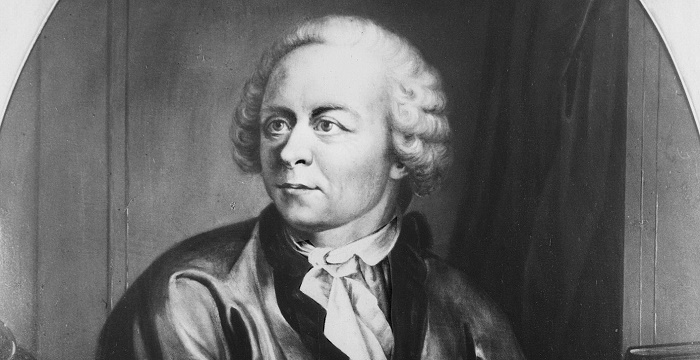
\includegraphics[width=14cm]{../resources/jpg/2.4.sequences.and.summations/euler.jpg}
    \caption*{Leonard Euler.}
\end{figure}    
\subsection[Lambda divided by lambda plus one is telescopic.]{
    \color{section} Theorem 100. \color{black} Lambda over lambda plus 1 is telescopic
}
\vspace{-0.8cm}
\documentclass[preview]{standalone}
\usepackage{amssymb, amsthm}
\usepackage{mathtools}
\usepackage{bm}


\newtheorem{theorem}{Theorem}
\renewcommand\qedsymbol{$\blacksquare$}


\begin{document}


\begin{theorem}[\textbf{2420}]
    \begin{equation*}
        \bm{
            \sum_{\epsilon=1}^\lambda 
                    \bigg \langle 
                        \frac{1}{\epsilon [ \epsilon + 1 ]}
                    \bigg \rangle
                = 
            \frac{\lambda}{\lambda + 1}
        }
    \end{equation*}
\end{theorem}

\begin{proof}
    The identity \bm{$\Big \langle \frac{1}{\epsilon [ \epsilon + 1 ]} \Big \rangle$} is 
    \bm{$\Big \langle \frac{1}{\epsilon} - \frac{1}{[ \epsilon + 1 ]} \Big \rangle$}. 
    This can be demonstrated by the equation
    \begin{equation*}
        \epsilon \bigg \langle \frac{1}{\epsilon} - \frac{1}{ [ \epsilon + 1 ] } \bigg \rangle 
            = 
        \bigg \langle \frac{\epsilon + 1}{\epsilon + 1} - \frac{\epsilon}{\epsilon + 1} \bigg \rangle
            = 
        \bigg \langle \frac{\epsilon + 1 - \epsilon}{\epsilon + 1} \bigg \rangle
            = 
        \bigg \langle \frac{1}{\epsilon + 1} \bigg \rangle
    \end{equation*}
    Dividing both sides of this equation by \bm{$\epsilon$},
    by the inverse law for multiplication from the field axioms,
    gives the desired identity such that
    \begin{equation*}
        \bigg \langle 
        \sum_{\epsilon=1}^\lambda 
                %\bigg \langle 
                    \frac{1}{\epsilon [ \epsilon + 1 ]}
                \bigg \rangle 
            = 
        \bigg \langle 
        \sum_{\epsilon=1}^\lambda 
                %\bigg \langle 
                    \frac{1}{\epsilon} - \frac{1}{\epsilon + 1} 
                \bigg \rangle
    \end{equation*}
    The sequence for which is the telescopic summation
    \begin{equation*}
        \bigg \langle \frac{1}{\lambda} - \frac{1}{\lambda + 1} \bigg \rangle
            + 
        \bigg \langle \frac{1}{\lambda - 1} - \frac{1}{\lambda} \bigg \rangle 
            + 
        \bigg \langle \frac{1}{\lambda - 2} - \frac{1}{\lambda - 1} \bigg \rangle
            + 
        \dots 
            + 
        \bigg \langle \frac{1}{1} - \frac{1}{2} \bigg \rangle
    \end{equation*}
    Thus, by Theorem 99
    \begin{equation*}
        \bm{
            \bigg \langle
            \sum_{\epsilon=1}^\lambda
                    %\bigg \langle
                        \frac{1}{ \epsilon [ \epsilon + 1 ] } 
                    \bigg \rangle
                = 
            \bigg \langle -\frac{1}{\lambda + 1} + \frac{1}{1} \bigg \rangle 
                = 
            \bigg \langle \frac{ [ -1 ] + [ \lambda + 1 ] }{\lambda + 1} \bigg \rangle 
                = 
            \frac{\lambda}{\lambda+1}
        }
    \end{equation*}
\end{proof}


\end{document}
\pagebreak


% ============================= 0101 Theorem 2421a ================================
\begin{figure}[!h]
    \centering
    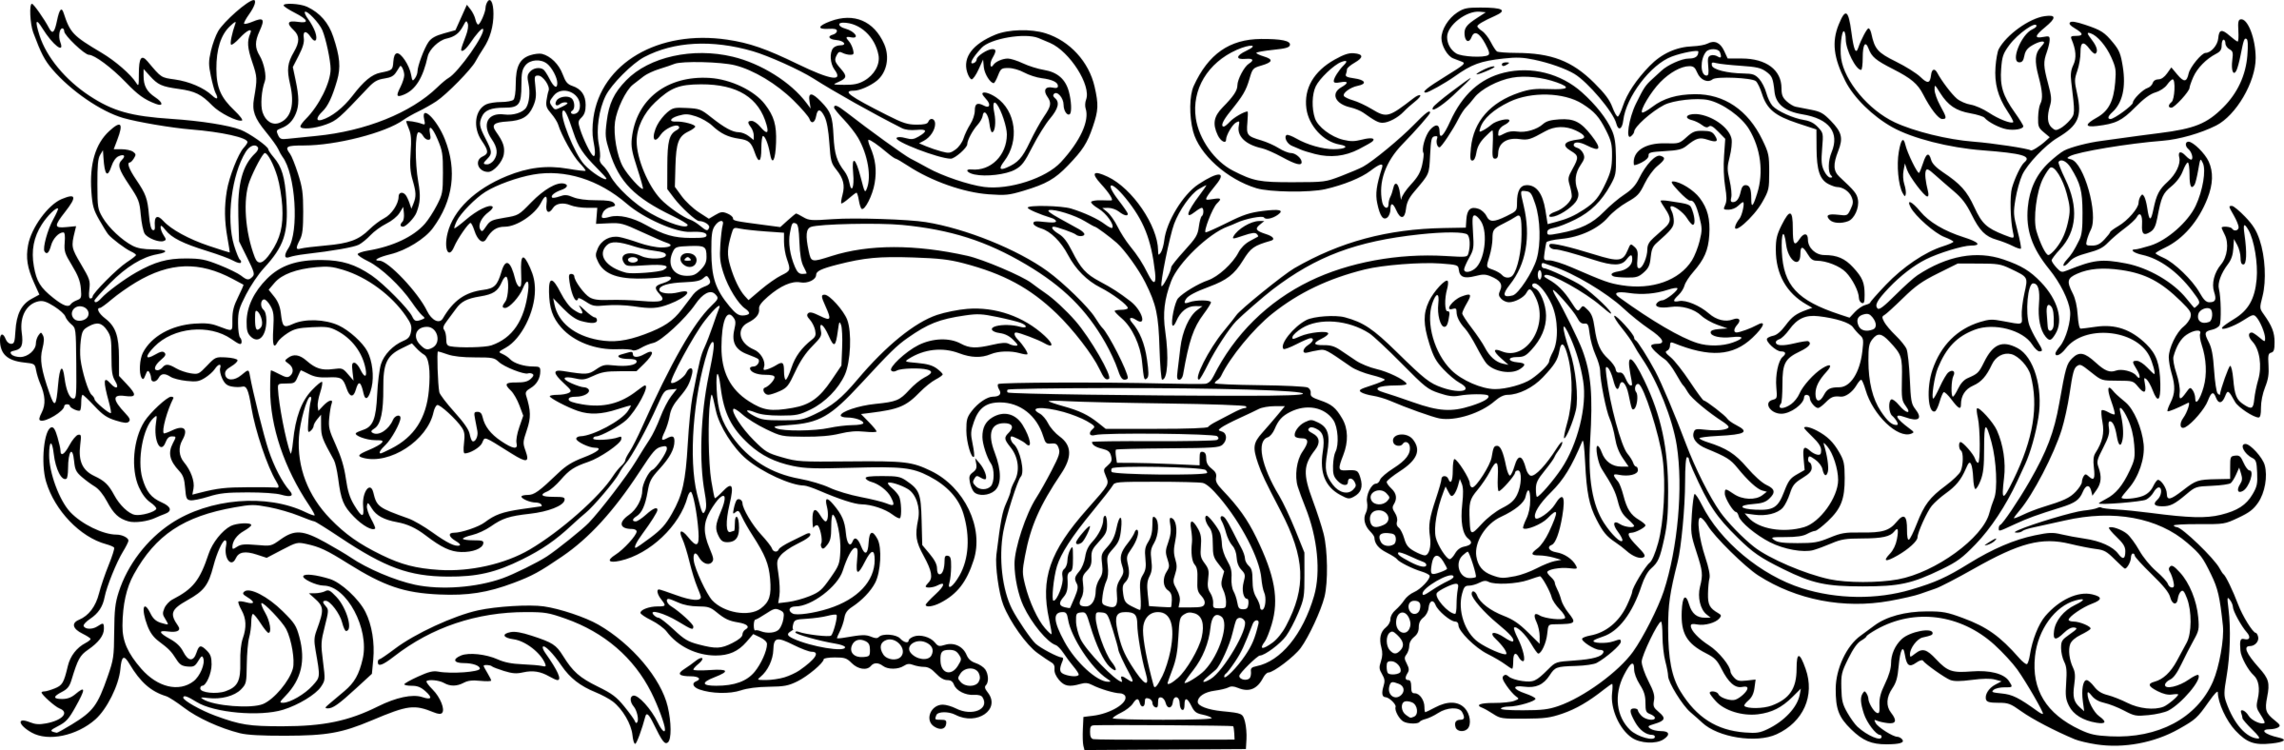
\includegraphics[width=14cm]{../resources/jpg/2.4.sequences.and.summations/border1.png}
\end{figure}
\subsection[The summation of odd numbers is a square.]{
    \color{section} Theorem 101. \color{black} The summation of odd numbers.
}
\documentclass[preview]{standalone}
\usepackage{amssymb, amsthm}
\usepackage{mathtools}
\usepackage{bm}


\newtheorem{theorem}{Theorem}
\renewcommand\qedsymbol{$\blacksquare$}


\begin{document}


\begin{theorem}[\textbf{2421a}]
    The summation of odd numbers from \bm{$1$} to \bm{$\phi$} is 
    \bm{$\phi^{2}$}.
\end{theorem}

\begin{proof}
    There exists an integer \bm{$\lambda$}, by the definition of odd numbers, such that
    the summation of odd numbers from \bm{$1$} to \bm{$\phi$} is given by, 
    \begin{equation*}
        \sum_{\lambda=1}^\phi 
                2 \lambda - 1
    \end{equation*}
    The identity for \bm{$2 \lambda - 1$} is the difference of squares 
    \bm{$\lambda ^2 - \big \langle \lambda - 1 \big \rangle ^2$}. 
    This identity can be demonstrated by the statement 
    \begin{equation*}
        \bigg \langle \lambda ^2 - [ \lambda - 1 ] ^2 \bigg \rangle
            = 
        \bigg \langle 
            \bigg[ 
                \lambda  + \langle \lambda - 1 \rangle 
            \bigg]
            \bigg[
                \lambda - \langle \lambda - 1 \rangle 
            \bigg] 
        \bigg \rangle
            =
    \end{equation*}
    \begin{equation*} 
        \bigg \langle 
            \bigg[
                2 \lambda - 1
            \bigg]
            \bigg[
                \lambda + \langle - \lambda + 1 \rangle
            \bigg]
        \bigg \rangle
            = 
        \bigg \langle [ 2 \lambda - 1 ] 1 \bigg \rangle
    \end{equation*}
    So the summation of odd numbers from \bm{$1$} to \bm{$\phi$} 
    is the telescoping summation
    \begin{equation*}
        \sum_{\lambda=1}^\phi 
                \lambda ^2 - \langle \lambda - 1 \rangle ^2
    \end{equation*}
    By Theorem 99, that is \bm{$\phi ^2 - 0 ^2 = \phi ^2$}. 
    Thus, 
    \begin{equation*}
        \sum_{\lambda=1}^\phi 2 \lambda - 1 = \phi^2
    \end{equation*}
    and indeed the summation of odd numbers from \bm{$1$} to \bm{$\phi$} 
    is \bm{$\phi ^2$}.
\end{proof}


\end{document}
\pagebreak

% ============================= 0102 Theorem 2421b ================================
\begin{figure}[!h]
    \centering
    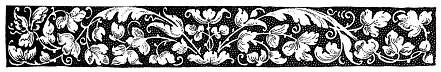
\includegraphics[width=14cm]{../resources/jpg/2.4.sequences.and.summations/border2.jpg}
\end{figure}
\subsection[The summation of natural numbers.]{
    \color{section} Theorem 102. \color{black} The summation of natural numbers.
}
\documentclass[preview]{standalone}
\usepackage{amssymb, amsthm}
\usepackage{mathtools}
\usepackage{bm}


\newtheorem{theorem}{Theorem}
\renewcommand\qedsymbol{$\blacksquare$}


\begin{document}


\begin{theorem}[\textbf{2421b}]
    The summation of natural numbers from \bm{$1$} to \bm{$\lambda$} 
    is 
    \begin{equation*}
        \bm{
            \frac{ \lambda [ \lambda + 1 ]}{2}
        }
    \end{equation*}
\end{theorem}

\begin{proof}
    It is possible to derive the closed formula for the summation of natural numbers
    from \bm{$1$} to \bm{$\lambda$} 
    from the summation of odd numbers from \bm{$1$} to \bm{$\lambda$}.
    By the definition for odd numbers, 
    an integer \bm{$\phi$} exists such that,
    by Theorem 101
    \begin{equation*}
        \sum_{\phi=1}^\lambda 2 \phi - 1 
            = 
        \lambda ^2
    \end{equation*}
    By the associative law for addition from the field axioms,
    \begin{equation*}
        \bigg \langle \sum_{\phi=1}^\lambda 2 \phi - 1 \bigg \rangle
            \equiv
        \bigg \langle 
            \sum_{\phi=1}^\lambda 2 \phi 
                +
            \sum_{\phi=1}^\lambda - 1
        \bigg \rangle
            \equiv
        \bigg \langle 
            -\lambda 
                +
            \sum_{\phi=1}^\lambda 2 \phi 
        \bigg \rangle
    \end{equation*}
    Thus, by that identity, and by the inverse law for addition from the field axioms,
    \begin{equation*}
        \Bigg\{
            \bigg \langle \lambda ^2 \bigg \rangle
                = 
            \bigg \langle 
                -\lambda 
                    + 
                \sum_{\phi=1}^\lambda 2 \phi 
            \bigg \rangle
        \Bigg\}
            \equiv 
        \Bigg\{
            \bigg \langle \sum_{\phi=1}^\lambda 2 \phi \bigg \rangle 
                = 
            \bigg \langle \lambda ^2 + \lambda \bigg \rangle 
                = 
            \lambda \bigg \langle \lambda + 1 \bigg \rangle
        \Bigg\}
    \end{equation*}
    By the distributive laws for real numbers from the field axioms, that is
    \begin{equation*}
        2 \sum_{\phi=1}^\lambda \phi 
            = 
        \lambda \Big \langle \lambda + 1 \Big \rangle
    \end{equation*} 
    And by the inverse law for multiplication from the field axioms,
    \begin{equation*}
        \bm{
            \sum_{\phi=1}^\lambda \phi 
                = 
            \frac{ \lambda [ \lambda + 1 ] }{2}
        }
    \end{equation*}
\end{proof}


\end{document}
\pagebreak


% ============================== 0103 Theorem 2422 ================================
\subsection[The summation of squares.]{
    \color{section} Theorem 103. \color{black} The summation of squares.
}
\documentclass[preview]{standalone}
\usepackage{amssymb, amsthm}
\usepackage{mathtools}
\usepackage{bm}


\newtheorem{theorem}{Theorem}
\renewcommand\qedsymbol{$\blacksquare$}


\begin{document}


\begin{theorem}[\textbf{2422}]
    The sum of squares from \bm{$1$} to \bm{$\lambda$} is 
    \begin{equation*}
        \bm{
            \frac{ 
                \lambda 
                \langle \lambda + 1 \rangle 
                \langle 2 \lambda + 1 \rangle 
            }
            {6}
        }
    \end{equation*}
\end{theorem}

\begin{proof}
    The formula for the summation of squares 
    from \bm{$1$} to \bm{$\lambda$} 
    can be derived from the cube of \bm{$\lambda$}.
    It is trivial that 
    \bm{$\lambda ^3 = \lambda ^3 - \big \langle 1 - 1 \big \rangle ^3$}. 
    By this identity for \bm{$\lambda$},
    the cube of \bm{$\lambda$} is the telescopic summation given by Theorem 2419, 
    \begin{equation*}
        \lambda ^3 
            = 
        \sum_{\iota=1}^\lambda \iota ^3 - \big \langle \iota - 1 \big \rangle ^3    
    \end{equation*}
    The expansion for 
    \bm{$\big \langle \iota - 1 \big \rangle ^3$} 
    is 
    \bm{$\iota ^3 - 3 \iota ^2 + 3 \iota - 1$}, 
    by the Binomial Theorem. 
    Thus, 
    by the inverse law for addition from the field axioms,
    yielding the algebraic identity
    \begin{equation*}
        \iota ^3 - \big \langle \iota - 1 \big \rangle ^3 
            = 
        3 \iota ^2 - 3 \iota + 1
    \end{equation*}
    Hence, 
    \bm{$\lambda ^3 = \sum_{\iota=1}^\lambda 3 \iota ^2 - 3 \iota + 1$}.
    By the commutative law for addition from the field axioms, 
    and by the distributive law for real numbers,
    that is
    \begin{equation*}
        \lambda ^3 
            = 
        \left( 3 \sum_{\iota=1}^\lambda \iota ^2 \right) 
            - 
        \left( 3 \sum_{\iota=1}^\lambda \iota \right) 
            + 
        \left( \sum_{\iota=1}^\lambda 1 \right)
    \end{equation*}
    Note that \bm{$
        \sum_{\iota=1} ^\lambda 1 
            = 
        \lambda \big \langle 1 \big \rangle
    $}. 
    And by Theorem 2421b, 
    \bm{$
        \sum_{\iota=1}^\lambda \iota 
            = 
        \frac{ \lambda \big \langle \lambda + 1 \big \rangle }{2}
    $}. 
    Thus, 
    by those identities, 
    and by the inverse law for addition from the field axioms
    \begin{equation*}
        \lambda ^3 
            + 
        3 \frac{ \lambda \big \langle \lambda + 1 \big \rangle }
        {2} 
            - 
        \lambda 
            = 
        3 \sum_{\iota=1}^\lambda \iota ^2
    \end{equation*}
    Eliminating the coefficient \bm{$3$} from the right-hand side, 
    by the inverse law for multiplication from the field axioms, 
    gives us the sum of squares in terms of an equation, 
    \begin{equation*}
        \frac{1}{3}
        \bigg[
            \lambda ^3 
                + 
            3 \frac{ \lambda \big \langle \lambda + 1 \big \rangle }
            {2} 
                - 
            \lambda
        \bigg]
            = 
        \sum_{\iota=1}^\lambda \iota ^2
    \end{equation*}
    By Lemma 2401, that is
    \begin{equation*}
        \bm{
            \sum_{\iota=1}^\lambda \iota ^2 
                = 
            \frac{ 
                \lambda \big \langle \lambda + 1 \big \rangle
                \big \langle 2 \lambda + 1 \big \rangle 
            }
            {6}
        }
    \end{equation*}
\end{proof}


\end{document}
\sep
\pagebreak


% ============================== 0104 Theorem 2425 ================================
\subsection[The summation of floors of square roots.]{
    \color{section} Theorem 104. \color{black} The summation of floors of square roots.
}
\documentclass[preview]{standalone}
\usepackage{amssymb, amsthm}
\usepackage{mathtools}
\usepackage{bm}


\newtheorem{theorem}{Theorem}
\renewcommand\qedsymbol{$\blacksquare$}


\begin{document}


\begin{theorem}[\textbf{2425}]
    
    \raggedright Let \bm{$\phi$} be a positive integer such that
    \raggedright \bm{$\lfloor \sqrt \phi \rfloor = \lambda$}.
    \raggedright The closed form formula for 
    \raggedright \bm{$
        \Phi
            = 
        \sum_{\iota=0}^\phi 
                \big \lfloor \sqrt \iota \big \rfloor
    $} 
    is 
    \begin{equation*}
        \bm{
            \frac{
                \lambda
                \big \langle \lambda - 1 \big \rangle
            }
            {6}
            \Bigg[
                4 \lambda + 1
            \Bigg]
                +
            \lambda
            \Bigg[
                \phi
                    -
                \lambda ^2
                    +
                1
            \Bigg]
        }
    \end{equation*}
\end{theorem}

\begin{proof}
    By the associative law for addition from the field axioms,
    \begin{equation*}
        \Theta
            = 
        \sum_{\iota=0}^{\lambda - 1} 
                \big \lfloor \sqrt \iota \big \rfloor 
            =
    \end{equation*}
    \begin{equation*}
        \Bigg (
            \sum_{\iota=1}^{ 2 \beta_0 + 1 } 
                    \big \lfloor \sqrt \iota \big \rfloor_0 
        \Bigg )
            +
        \Bigg (
            \sum_{\iota=1 + 2 \beta_0 + 1}^{ 2 \beta_0 + 1 + 2 \beta_1 + 1 } 
                    \big \lfloor \sqrt \iota \big \rfloor_1 
        \Bigg )
            +
        \dots
            +
        \Bigg (
            \sum_{\iota=1 +  \dots + 2 \beta_{\langle \lambda - 2 \rangle} + 1 }
                ^{0 + \dots + 2 \beta_{\langle \lambda - 1 \rangle} + 1} 
                    \big \lfloor \sqrt \iota \big \rfloor_{
                        \langle \lambda - 1 \rangle
                    } 
        \Bigg )
    \end{equation*}
    \bm{$\big \lfloor \sqrt \iota \big \rfloor_\tau$}
    is the unique integer \bm{$\beta_\tau$}, 
    for \bm{$\tau = 0$} to \bm{$\big \langle \lambda - 1 \big \rangle$}.
    Hence, by Lemma 12 and the distributive law for real numbers from the field axioms, 
    by the partitioning from above, and shifting the index of summation,
    \begin{equation*}
        \Theta
            =
        \Big \langle 2 \beta_{0} ^2 + \beta_0 \Big \rangle
            +
        \Big \langle 2 \beta_{1} ^2 + \beta_1 \Big \rangle
            +
        \dots
            +
        \Big \langle 
            2 \beta_{[ \lambda - 1 ]} ^2
                +
            \beta_{[ \lambda - 1 ]}
        \Big \rangle
    \end{equation*}
    By the commutative law for addition from the field axioms,
    that series is two times the finite summation of squares, 
    plus the finite summation of integers from zero to lambda minus one.
    \begin{equation*}
        \Theta
            = 
        \sum_{\tau=0}^{ \lambda - 1 } 2 \tau ^2 
            +
        \sum_{\tau=0}^{ \lambda - 1 } \tau
    \end{equation*}
    Lambda occurs exactly 
    \bm{$
        \big \langle 
            \phi - \lambda ^2 + 1
        \big \rangle
    $} 
    times in big phi.
    Thus, by Lemma 11 and the distributive law for real numbers from the field axioms,
    \begin{equation*}
        \bm{
            \Phi
                =
            \frac{
                \lambda
                \big \langle \lambda - 1 \big \rangle
            }
            {6}
            \Bigg[
                4 \lambda + 1
            \Bigg]
                +
            \lambda
            \Bigg[
                \phi
                    -
                \lambda ^2
                    +
                1
            \Bigg]
        }
    \end{equation*}
\end{proof}


\end{document}
\begin{figure}[!h]
    \centering
    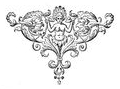
\includegraphics[width=3cm]{../resources/jpg/2.4.sequences.and.summations/symbol6.jpg}
\end{figure}
\pagebreak

% ============================== 0105 Theorem 2426 ================================
\subsection[The summation of floors of cube roots.]{
    \color{section} Theorem 105. \color{black} The summation of floors of cube roots.
}
\documentclass[preview]{standalone}
\usepackage{amssymb, amsthm}
\usepackage{mathtools}
\usepackage{bm}


\newtheorem{theorem}{Theorem}
\renewcommand\qedsymbol{$\blacksquare$}


\begin{document}


\begin{theorem}[\textbf{2426}]
    \raggedright Let \bm{$\phi$} be a positive integer such that 
    \raggedright \bm{$\big \lfloor \sqrt[3] \phi \big \rfloor = \lambda$}.
    \raggedright The closed form formula for 
    \raggedright \bm{
        $\Phi = \sum_{\iota=0}^\phi 
                \big \lfloor \sqrt[3] \iota \big \rfloor
    $} 
    is 
    \begin{equation*}
        \bm{
            \frac{
                \lambda ^3 - \lambda ^2
            }
            {4}
            \Bigg[ 3 \lambda + 1 \Bigg]
                + 
            \lambda
            \Bigg[
                \phi - \lambda ^3 + 1
            \Bigg]
        }
    \end{equation*}
\end{theorem}

\begin{proof}
    Let \bm{$\mathrm{X}$} be the function 
    \bm{$\mathrm{X}: \mathbb{N} \rightarrow \mathbb{N}$}
    such that \bm{$\mathrm{X}[\beta] = 3 \beta ^2 + 3 \beta + 1$}.
    By the associative law for addition from the field axioms,
    \begin{equation*}
        \Theta
            =
        \sum_{\iota=0}^{\lambda - 1}
                \big \lfloor \sqrt[3] \iota \big \rfloor
            =
    \end{equation*}
    \begin{equation*}
        \Bigg(
            \sum_{ \iota = 1 }^{ \mathrm{X} [\beta_0] }
                \big \lfloor \sqrt[3] \iota \big \rfloor_0
        \Bigg)
            +
        \Bigg(
            \sum_{
                \iota = 1 + \mathrm{X}[\beta_0]
            }^{ 
                \mathrm{X}[\beta_0] + \mathrm{X}[\beta_1]
            }
                \big \lfloor \sqrt[3] \iota \big \rfloor_1
        \Bigg)
            +
        \dots
            +
        \Bigg(
            \sum_{
                \iota = 1 + \dots 
                    + 
                \mathrm{X}[\beta_{\lambda - 2}]
            }^{ 
                0 + \dots
                    +
                \mathrm{X}[\beta_{ \lambda - 1 }]
            }
                \big \lfloor \sqrt[3] \iota \big \rfloor_{ \langle \lambda - 1 \rangle }
        \Bigg)
    \end{equation*}
    \bm{$\big \lfloor \sqrt[3] \iota \big \rfloor_\tau$}
    is the unique integer \bm{$\beta_\tau$},
    for \bm{$\tau = 0$} to 
    \bm{$\big \langle \lambda - 1 \big \rangle$}.
    Hence, by Lemma 13,
    by the partitioning from above, 
    and shifting the index of summation,
    \begin{equation*}
        \Theta
            =
        \Big \langle \beta_0 \mathrm{X} [\beta_0] \Big \rangle
            +
        \Big \langle \beta_1 \mathrm{X} [\beta_1] \Big \rangle
            + 
        \dots 
            +
        \Big \langle 
            \beta_{\langle \lambda - 1 \rangle}
            \mathrm{X} [\beta_{\langle \lambda - 1 \rangle}]
        \Big \rangle
    \end{equation*}
    By the distributive law for real numbers from the field axioms,
    and the commutative law for addition, that series is
    three times the finite summation of cubes,
    plus three times the finite summation of squares,
    plus the finite summation of integers from zero to lambda minus one.
    \begin{equation*}
        \Theta 
            = 
        \sum_{\tau=0}^{\lambda - 1} 3 \tau ^3
            +
        \sum_{\tau=0}^{\lambda - 1} 3 \tau ^2
            +
        \sum_{\tau=0}^{\lambda - 1} \tau
    \end{equation*}
    Lambda occurs exactly  
    \bm{$\big \langle \phi - \lambda^3 + 1 \big \rangle$}
    times in big phi. 
    Thus, by Lemma 14
    and the distributive law for real numbers from the field axioms,
    \begin{equation*}
        \bm{
            \Phi
                =
            \frac{
                \lambda ^3 - \lambda ^2
            }
            {4}
            \Bigg[ 3 \lambda + 1 \Bigg]
                + 
            \lambda
            \Bigg[
                \phi - \lambda ^3 + 1
            \Bigg]
        }
    \end{equation*}
\end{proof}


\end{document}
\begin{figure}[!h]
    \centering
    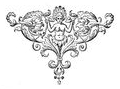
\includegraphics[width=3cm]{../resources/jpg/2.4.sequences.and.summations/symbol6.jpg}
\end{figure}
\pagebreak


% ============================== 0106 Theorem 2436 ================================
\subsection[Subsets of countable sets are countable.]{
    \color{section} Theorem 106. \color{black} Subsets of countable sets are countable.
}
\documentclass[preview]{standalone}
\usepackage{amssymb, amsthm}
\usepackage{mathtools}
\usepackage{bm}


\newtheorem{theorem}{Theorem}
\renewcommand\qedsymbol{$\blacksquare$}


\begin{document}


\begin{theorem}[\textbf{2436}]
    A subset of a countable set is countable.
\end{theorem}

\begin{proof}
    Let \bm{$\mathrm{A}$} and \bm{$\Lambda$} be sets such that 
    \bm{$\mathrm{A}$} is a subset of the countable set \bm{$\Lambda$}. 
    By the definition for countability,
    the cardinality of \bm{$\Lambda$} is less than or equal to \bm{$\aleph_0$}. 
    By the definition for subsets, 
    the cardinality of \bm{$\mathrm{A}$}
    is less than or equal to \bm{$\Lambda$}.
    Hence,
    the cardinality of \bm{$\mathrm{A}$} is less than or equal to \bm{$\aleph_0$}
    \bm{$\therefore$} the subset of a countable set is countable.
\end{proof}


\end{document}
\sep


% ============================== 0107 Theorem 2437 ================================
\subsection[Uncountable subsets imply an uncountable superset.]{
    \color{section} Theorem 107. \color{black} Uncountable subsets.
}
\documentclass[preview]{standalone}
\usepackage{amssymb, amsthm}
\usepackage{mathtools}
\usepackage{bm}


\newtheorem{theorem}{Theorem}
\renewcommand\qedsymbol{$\blacksquare$}


\begin{document}


\begin{theorem}[\textbf{2437}]
    Let \bm{$\mathrm{A}$}, and \bm{$\Lambda$} be sets such that 
    \bm{$\mathrm{A}$} is a subset of \bm{$\Lambda$}. 
    If \bm{$\mathrm{A}$} is uncountable, 
    then \bm{$\Lambda$} is uncountable.
\end{theorem}

\begin{proof}
    Direct proof.
    The cardinality for \bm{$\mathrm{A}$} is greater than \bm{$\aleph_0$},
    by the definition for countability. 
    By the definition of subsets, 
    the cardinality of \bm{$\Lambda$} is at least the cardinality 
    of \bm{$\mathrm{A}$}. 
    Hence, \bm{$\Lambda$} is uncountable, by the definition for countability.
\end{proof}


\end{document}
\sep


% ============================== 0108 Theorem 2438 ================================
\subsection[Power set cardinality.]{
    \color{section} Theorem 108. \color{black} Power set cardinality.
}
\documentclass[preview]{standalone}
\usepackage{amssymb, amsthm}
\usepackage{mathtools}
\usepackage{bm}


\newtheorem{theorem}{Theorem}
\renewcommand\qedsymbol{$\blacksquare$}


\begin{document}


\begin{theorem}[\textbf{2438}]
    Let \bm{$\mathrm{A}$}, and \bm{$\Lambda$} be sets with equal cardinality. 
    \begin{equation*}
        \bm{
            \Big| 
                \mathcal{P}\big \langle \mathrm{A} \big \rangle 
            \Big| 
                = 
            \Big|
                \mathcal{P} \big \langle \Lambda \big \rangle 
            \Big|
        }
    \end{equation*}
\end{theorem}

\begin{proof}
    By the hypothesis, and by the defintion for set cardinality,
    there exists an integer \bm{$\iota$} such that 
    \bm{$
        \big| \mathrm{A} \big| 
            = 
        \big| \Lambda \big| 
            = \iota
    $}. 
    The cardinality of a power set is $2$ to the power of the set cardinality. 
    Thus,
    \begin{equation*}
        \bm{
            \big | \mathcal{P} \big \langle \mathrm{A} \big \rangle \big | 
                = 
            \big | \mathcal{P} \big \langle \Lambda \big \rangle \big | 
                = 
            2^{\iota}
        }        
    \end{equation*} 
\end{proof}


\end{document}
\begin{figure}[!h]
    \centering
    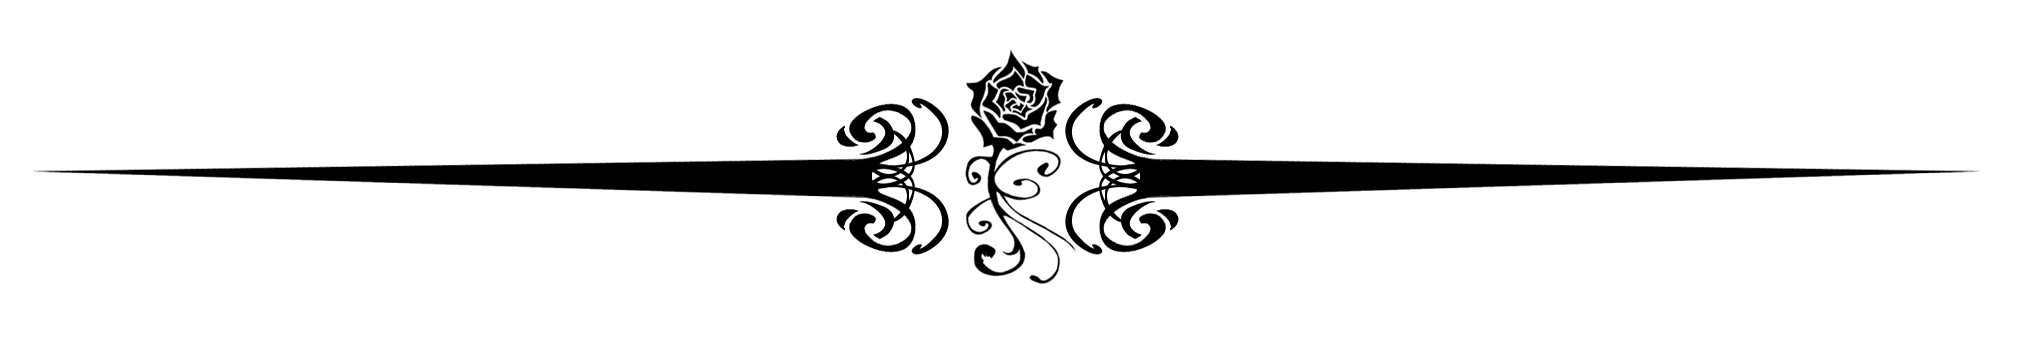
\includegraphics[width=4cm]{../resources/jpg/2.4.sequences.and.summations/border.png}
\end{figure}
\pagebreak


% ============================== 0109 Theorem 2440 ================================
\subsection[Union of countable sets is countable.]{
    \color{section} Theorem 109. \color{black} Union of countable sets is countable.
}
\documentclass[preview]{standalone}
\usepackage{amssymb, amsthm}
\usepackage{mathtools}
\usepackage{bm}


\newtheorem{theorem}{Theorem}
\renewcommand\qedsymbol{$\blacksquare$}


\begin{document}


\begin{theorem}[\textbf{2440}]
    The union of two countable sets is countable.
\end{theorem}

\begin{proof}
    By cases. Let \bm{$\mathrm{A}$}, and \bm{$\Lambda$} be countable sets. 
    There are three possible cases. 
    $(i)$ \bm{$\mathrm{A}$} and \bm{$\Lambda$} are finite, 
    $(ii)$ exclusively \bm{$\mathrm{A}$} or \bm{$\Lambda$} is finite and the other is countably infinite, 
    $(iii)$ \bm{$\mathrm{A}$} and \bm{$\Lambda$} are both countably infinite.
    \\ \\
    \bm{$(i)$} Assume \bm{$\mathrm{A}$} and \bm{$\Lambda$} are finite. 
    There exist natural numbers \bm{$\lambda$}, and \bm{$\iota$} such that 
    \bm{$\big |\mathrm{A} \big | = \lambda$} and 
    \bm{$\big | \Lambda \big | = \iota$}. 
    The maximum cardinality for \bm{$\mathrm{A} \cup \Lambda$} 
    occurs when the intersection of \bm{$\mathrm{A}$} and \bm{$\Lambda$} is 
    the empty set. The cardinality for such a union is \bm{$\lambda + \iota$}. 
    \bm{$\lambda + \iota$} is a natural number by the closure property for addition on integers. 
    Thus, \bm{$\lambda + \iota$} is less than \bm{$\aleph_0$}. 
    By the definition for countably finite sets, \bm{$\mathrm{A} \cup \Lambda$} is countable. 
    \\ \\
    \bm{$(ii)$} Without loss of generality assume \bm{$\mathrm{A}$} is finite with cardinality \bm{$\lambda$}, 
    and \bm{$\Lambda$} is countably infinite. 
    A finite sequence 
    \bm{$\big \{ \alpha_\iota \big \}$}
    containing all members of \bm{$\mathrm{A}$},
    and an infinite sequence 
    \bm{$\big \{ \beta_{ \mathbb{N} } \big \}$}
    containing all members of \bm{$\Lambda$}
    exists.
    For the union of \bm{$\mathrm{A}$} and \bm{$\Lambda$} 
    there exists a sequence \bm{$ \big \{ \delta \big \} $} such that
    \begin{equation*}
        \{ 
            \delta_\mathbb{N} 
        \} 
            = 
        \{\alpha_0, \alpha_1, \dots, \alpha_\lambda, 
        \beta_{\lambda+1}, \beta_{\lambda +2}, \beta_{\lambda + 3}, \dots \}
    \end{equation*}
    Clearly this is countably infinite by the definition for countability 
    since \bm{$\lambda + \chi$} is a natural number 
    for all \bm{$\chi$} in natural numbers, 
    by the closure property for addition on natural numbers. 
    \\ \\
    \bm{$(iii)$} assume both \bm{$\mathrm{A}$} and \bm{$\Lambda$} are countable infinite sets. 
    Since each set cardinality is \bm{$\aleph_0$}, 
    an infinite sequence 
    \bm{$\big \{ \alpha_\mathbb{N} \big \}$}
    containing all members of \bm{$\mathrm{A}$},
    and an infinite sequence 
    \bm{$\big \{ \beta_{ \mathbb{N} } \big \}$}
    containing all members of \bm{$\Lambda$}
    exist.
    For the union of \bm{$\mathrm{A}$} and \bm{$\Lambda$}
    there exists a infinite sequence \bm{$\big \{ \delta \big \} $} such that
    \begin{equation*}
        \big \{ \delta_\mathbb{N} \big \} 
            = 
        \big \{
            \alpha_{0_0}, \beta_{0_1}, 
            \alpha_{1_2}, \beta_{1_3}, 
            \alpha_{2_4}, \beta_{2_5}, 
            \dots
        \big \}    
    \end{equation*}
    Thus a bijection 
    exists between \bm{$\mathbb{N}$} and the union of \bm{$\mathrm{A}$} and \bm{$\Lambda$}, 
    and that union is countable by the definition for countability.
\end{proof}


\end{document}
\vspace{1\baselineskip}
\begin{figure}[!h]
    \centering
    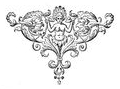
\includegraphics[width=3cm]{../resources/jpg/2.4.sequences.and.summations/symbol6.jpg}
\end{figure}
\pagebreak


% ============================== 0110 Theorem 2441 ================================
\begin{figure}[!h]
    \centering
    
\includegraphics[width=14cm]{../resources/jpg/2.4.sequences.and.summations/infinity.jpg}
\end{figure}
\subsection[A countable union of countable sets is countable.]{
    \color{section} Theorem 110. \color{black} A countable union.
}
\documentclass[preview]{standalone}
\usepackage{amssymb, amsthm}
\usepackage{mathtools}
\usepackage{bm}


\newtheorem{theorem}{Theorem}
\renewcommand\qedsymbol{$\blacksquare$}


\begin{document}


\begin{theorem}[\textbf{2441}]
    The union of a countable number of countable sets is countable.
\end{theorem}

\begin{proof}
    Let $A_i$ be a countable set, for integers $i=0$ to $n \leq \infty$ 
    such that
    $$S = \bigcup_{i=0}^{n} A_i$$ 
    The function $f: \mathbb{N} \rightarrow A_i$ is the sequence 
    $\{a_{ij}\} = a_{i0}, a_{i1}, a_{i2}, \dots$. 
    Thus, by $f$, all elements $a_{ij}$ in $S$ can be listed in the second dimension
    $$a_{00}, a_{01}, a_{02}, \dots$$
    $$a_{10}, a_{11}, a_{12}, \dots$$
    $$a_{20}, a_{21}, a_{22}, \dots$$
    $$\vdots$$
    By tracing the diagonal path along the two 
    dimensional listing for $S$ we get the countable order 
    $$a_{00}, a_{01}, a_{10}, a_{20}, a_{11}, a_{02}, \dots$$
    $\therefore |S| \leq \aleph_0$, and indeed the union of a countable number of 
    countable sets is countable.
\end{proof}


\end{document}
\pagebreak


% ============================== 0111 Theorem 2442 ================================
\subsection[The Cartesian product of positive integers.]{
    \color{section} Theorem 111. \color{black} The cross product of positive integers.
}
\documentclass[preview]{standalone}
\usepackage{amssymb, amsthm}
\usepackage{mathtools}
\usepackage{bm}


\newtheorem{theorem}{Theorem}
\renewcommand\qedsymbol{$\blacksquare$}


\begin{document}


\begin{theorem}[\textbf{2442}]
    The cardinality of $\mathbb{Z^{+}} \times \mathbb{Z^{+}}$ is aleph null.
\end{theorem}

\begin{proof}
    $\mathbb{Z^{+}} \times \mathbb{Z^{+}}$ is defined as 
    $\{ \langle x, y \rangle | (x \in \mathbb{Z^{+}}) \land (y \in \mathbb{Z^{+}})\}$. 
    Since $x$ and $y$ are positive integers, for every ordered pair $\langle x, y \rangle$ in 
    $\mathbb{Z^{+}} \times \mathbb{Z^{+}}$, $\langle x, y \rangle$ exists if and only if the rational number 
    $\frac{x}{y}$ exists. Thus, $\frac{x}{y}$ exists, and all elements in 
    $\mathbb{Z^{+}} \times \mathbb{Z^{+}}$ can be represented by the two dimensional list
    $$\langle 1,1 \rangle \iff \frac{1}{1}, \langle 1,2 \rangle \iff \frac{1}{2}, \langle 1,3 \rangle \iff \frac{1}{3}, \dots$$
    $$\langle 2,1 \rangle \iff \frac{2}{1}, \langle 2,2 \rangle \iff \frac{2}{2}, \langle 2,3 \rangle \iff \frac{2}{3}, \dots$$
    $$\langle 3,1 \rangle \iff \frac{3}{1}, \langle 3,2 \rangle \iff \frac{3}{2}, \langle 3,3 \rangle \iff \frac{3}{3}, \dots$$
    $$\vdots$$
    The hypotheses in the biconditional converse statements for each list entry are the list 
    elements in the proof for the countability of rational numbers. That means 
    $\mathbb{Z^{+}} \times \mathbb{Z^{+}}$ is countable if and only if the rational numbers are 
    countable. We know the rational numbers are countable. Therefore the cardinality of 
    $\mathbb{Z^{+}} \times \mathbb{Z^{+}}$ is $\aleph_0$.
\end{proof}


\end{document}
\sep


% ============================== 0112 Theorem 2443 ================================
\subsection[The set of all finite bit strings is countable.]{
    \color{section} Theorem 110. \color{black} The set of all finite bit strings.
}
\documentclass[preview]{standalone}
\usepackage{amssymb, amsthm}
\usepackage{mathtools}
\usepackage{bm}


\newtheorem{theorem}{Theorem}
\renewcommand\qedsymbol{$\blacksquare$}


\begin{document}


\begin{theorem}[\textbf{2443}]
    The set of all finite bit strings is countable.
\end{theorem}

\begin{proof}
    Let $\{a_{n-1}\}$ be the sequence of bits for any finite bit string $a($base-$2)$ of length $n$. 
    The unique base-$2$ expansion for $\{a_{n-1}\}$ is the integer
    $$a(\text{base-}10) = \sum_{i = 0}^{n-1} a_{i}2^{i}$$
    Also, this integer can be converted to the unique base-$2$ bit string for \\ $a($base-$10)$ by 
    $$a(\text{base-}2) = 
    \sum_{i = 0}^{n-1}\left[a(\text{base-}10)(\text{mod } 2^{i+1})\right]10^{i}$$ 
    Since an invertible function exists between each finite bit string and some positive integer, 
    there exists, a one-to-one correspondence between $\mathbb{Z}$ and the set of all 
    finite bit strings. Thus, the cardinality for the set of all finite bit strings is $\aleph_0$,
    and the set of all finite bit strings is countable, by definition.
\end{proof}


\end{document}


\section{Lemmas}
% ================================ 0010L Lemma 2401 =================================
\subsection[Lemma 10]{\color{section}Lemma 10}
\documentclass[preview]{standalone}
\usepackage{amssymb, amsthm}
\usepackage{mathtools}
\usepackage{bm}


\newtheorem{lemma}{Lemma}
\renewcommand\qedsymbol{$\blacksquare$}


\begin{document}


\begin{lemma}[\textbf{2401}]
    Let \bm{$\lambda$} be a positive integer.
    \begin{equation*}
        \bm{
            \frac{1}{3} 
            \bigg[ 
                \lambda^3 
                    + 
                3 \bigg \langle 
                    \frac{ \lambda [ \lambda + 1 ] }{2} 
                \bigg \rangle
                    - 
                    \lambda 
            \bigg] 
                =
            \bigg[
                \frac{
                    \lambda
                    \langle \lambda + 1 \rangle 
                    \langle 2 \lambda + 1 \rangle}
                    {6}
            \bigg]
        }
    \end{equation*}
\end{lemma}

\begin{proof}
    By the distributive laws for real numbers, 
    and by the associative law for multiplication,
    \begin{equation*}
        3 \bigg \langle \frac{ \lambda [ \lambda + 1 ] }{2} \bigg \rangle 
            = 
        \bigg \langle \frac{3 \lambda ^2 + 3 \lambda }{2} \bigg \rangle
    \end{equation*}
    Since the rational number \bm{$\frac{2}{2} = 1$} 
    by the inverse law for multiplication, 
    by the multiplicative identity law from the field axioms,
    (and by the identity established above,)
    \begin{equation*} 
            \bigg[ 
                \lambda ^3 
                    + 
                3 \bigg \langle \frac{ \lambda [ \lambda + 1 ] }{2} \bigg \rangle
                    - 
                \lambda 
            \bigg]
            =
            \bigg[
                \frac{ 2 \lambda ^3 }{2} \
                    + 
                \frac{ 3 \lambda ^2 + 3 \lambda }{2} 
                    - 
                \frac{ 2 \lambda }{2}
            \bigg]
    \end{equation*}
    By the distributive law for real numbers
    \begin{equation*}
            \frac{1}{3}
            \bigg[
                \frac{ 2 \lambda ^3 }{2} 
                    + 
                \frac{ 3 \lambda ^2 + 3 \lambda }{2} 
                    - 
                \frac{ 2 \lambda }{2}
            \bigg]
                =
            \bigg[
                \frac{ 2 \lambda ^3 + 3 \lambda ^2 + 3 \lambda - 2 \lambda }
                {6}
            \bigg]
    \end{equation*}
    Repeated factoring, 
    by the distributive laws for real numbers,
    completes the proof.
    \begin{equation*}
        \bigg[
            \frac{ 2 \lambda ^3 + 3 \lambda ^2 + 3 \lambda - 2 \lambda }{6}
        \bigg]
            =
        \bigg[
            \frac{ \lambda \langle 2 \lambda ^2 + 2 \lambda + \lambda + 1 \rangle }{6}
        \bigg]
            =
        \bigg[
            \frac{ \lambda \langle 2 \lambda [\lambda + 1] + [\lambda + 1] \rangle }{6}
        \bigg]
    \end{equation*}
    \begin{equation*}
            =
        \bm{
            \bigg[
                \frac{ \lambda \langle \lambda + 1 \rangle \langle 2 \lambda + 1 \rangle }{6}
            \bigg]
        }
    \end{equation*}
\end{proof}


\end{document}
\vspace{2\baselineskip}
\begin{figure}[!h]
    \centering
    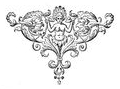
\includegraphics[width=3cm]{../resources/jpg/2.4.sequences.and.summations/symbol6.jpg}
\end{figure}
\pagebreak


% ================================ 0011L Lemma 2402 =================================
\subsection[Lemma 11]{\color{section}Lemma 11}
\documentclass[preview]{standalone}
\usepackage{amssymb, amsthm}
\usepackage{mathtools}
\usepackage{bm}


\newtheorem{lemma}{Lemma}
\renewcommand\qedsymbol{$\blacksquare$}


\begin{document}


\begin{lemma}[\textbf{2402}]
    Let \bm{$\iota$} be a positive integer such that
    \bm{$\big \lfloor \sqrt{\iota} \big \rfloor = \lambda$}.
    \begin{equation*}
        \bm{
            \Bigg( 2\sum_{\phi=0}^{\lambda - 1} \phi ^2 \Bigg)
                + 
            \Bigg( \sum_{\phi=0}^{\lambda - 1} \phi \Bigg)
                \equiv
            \frac{
                \lambda
                \big \langle \lambda - 1 \big \rangle
            }
            {6}
            \Bigg[
                4 \lambda + 1
            \Bigg]
        }
    \end{equation*}
\end{lemma}

\begin{proof}
    Let \bm{$\Phi$} be two times the sum of squares from zero to \bm{$\lambda$} minus one.
    Let \bm{$\mathrm{X}$} be the sum of integers from zero to \bm{$\lambda$} minus one.
    By theorems 103, and 102, and by shifting the index of summation,
    \begin{equation*}
        \Bigg\{
            \Phi + \mathrm{X}
        \Bigg\}
            \equiv
        2
        \Bigg[
            \frac{ 
                \lambda [ \lambda - 1 ]
                [ 2 \langle \lambda - 1 \rangle + 1 ] 
            }
            {6}
        \Bigg]
            +
        \Bigg[
            \frac{\lambda [ \lambda - 1 ] }
            {2}
        \Bigg]
    \end{equation*}
    Since the rational number \bm{$\frac{3}{3} = 1$}
    by the inverse law for multiplication,
    by the multiplicative identity law from the field axioms
    \begin{equation*}
        \bigg \{ \mathrm{X} \bigg\}   
            \equiv
        \frac{
            3
            \lambda [ \lambda - 1 ]
        }
        {6}
    \end{equation*}
    Thus, 
    by the identity \bm{$\mathrm{X}$}, 
    factoring
    \bm{$\frac{1}{6} \lambda \big \langle \lambda - 1 \big \rangle$}
    out from the sum of \bm{$\Phi$} and \bm{$\mathrm{X}$}, 
    by the distributive laws for real numbers,
    \begin{equation*}
        \Bigg\{
            \Phi
                +
            \mathrm{X}
        \Bigg\}
            \equiv
        \frac{
            \lambda
            \big \langle \lambda - 1 \big \rangle
        }
        {6}
        \Bigg[
            2 \bigg \langle 2 [ \lambda - 1 ] + 1 \bigg \rangle
                +
            3
        \Bigg]
    \end{equation*}
    By the distributive laws for real numbers, 
    and by the associative law for addition from the field axioms,
    \begin{equation*}
        \bigg \{
            2 \Big \langle 2 [ \lambda - 1 ] + 1 \Big \rangle + 3
        \bigg \}
            =
        \bigg \{
            4 [ \lambda - 1 \big ] + 5
        \bigg \}
            =
        \bigg \{
            4 \lambda + 1
        \bigg \}
    \end{equation*}
    \bm{$\therefore$}
    \begin{equation*}
        \bm{
            \Bigg \{
                \Phi
                    +
                \mathrm{X}
            \Bigg \}
                \equiv
            \frac{
                \lambda
                \big \langle \lambda - 1 \big \rangle
            }
            {6}
            \Bigg[
                4 \lambda + 1
            \Bigg]
        }
    \end{equation*}
\end{proof}


\end{document}
\begin{figure}[!h]
    \centering
    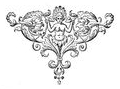
\includegraphics[width=3cm]{../resources/jpg/2.4.sequences.and.summations/symbol6.jpg}
\end{figure}
\pagebreak


% ================================ 0012L Lemma 2403 =================================
\subsection[Lemma 12]{\color{section}Lemma 12}
\documentclass[preview]{standalone}
\usepackage{amssymb, amsthm}
\usepackage{mathtools}
\usepackage{bm}


\newtheorem{lemma}{Lemma}
\renewcommand\qedsymbol{$\blacksquare$}


\begin{document}


\begin{lemma}[\textbf{2403}]
    Let \bm{$\iota$} be a natural number such that
    \bm{$\big \lfloor \sqrt \iota \big \rfloor = \lambda$}.
    \begin{equation*}
        \bm{
            \sum_{\iota=1}^{2 \lambda + 1} 
                    \big \lfloor \sqrt \iota \big \rfloor
                =
            \lambda \big[ 2 \lambda + 1 \big]
        }
    \end{equation*}
\end{lemma}

\begin{proof}
    It is trivial that
    \begin{equation*}
        \sum_{\iota=1}^{2 \lambda + 1} 
                1 = 2 \lambda + 1
    \end{equation*}
    By the inverse law for multiplication from the field axioms,
    by the distributive law for real numbers, and by the identity \bm{$\lambda$},
    that is
    \begin{equation*}
        \Bigg\{
            \lambda \sum_{\iota=1}^{2 \lambda + 1} 1 = \lambda \big[ 2 \lambda + 1 \big]
        \Bigg\}
                \equiv
        \Bigg\{
            \sum_{\iota=1}^{2 \lambda + 1} \lambda = \lambda \big[ 2 \lambda + 1 \big]
        \Bigg\}
            \equiv
        \Bigg\{
            \sum_{\iota=1}^{2 \lambda + 1} \big \lfloor \sqrt \iota \big \rfloor
                = 
            \lambda \big[ 2 \lambda + 1 \big]
        \Bigg\}
    \end{equation*}
\end{proof}


\end{document}
\sep


% ================================ 0013L Lemma 2404 =================================
\subsection[Lemma 13]{\color{section}Lemma 13}
\documentclass[preview]{standalone}
\usepackage{amssymb, amsthm}
\usepackage{mathtools}
\usepackage{bm}


\newtheorem{lemma}{Lemma}
\renewcommand\qedsymbol{$\blacksquare$}


\begin{document}


\begin{lemma}[\textbf{2404}]
    Let \bm{$\iota$} be a natural number such that
    \bm{$\big \lfloor \sqrt[3] \iota \big \rfloor = \lambda$}.
    \begin{equation*}
        \bm{
            \sum_{\iota=1}^{ 3 \lambda ^2 + 3 \lambda + 1 } 
                    \big \lfloor \sqrt[3] \iota \big \rfloor
                =
            \lambda \big [ 3 \lambda ^2 + 3 \lambda + 1 \big ]
        }
    \end{equation*}
\end{lemma}

\begin{proof}
    Similiar to Lemma 2403, it is trivial that
    \begin{equation*}
        \sum_{\iota=1}^{ 3 \lambda ^2 + 3 \lambda + 1 } 
                    1
                =
            3 \lambda ^2 + 3 \lambda + 1
    \end{equation*}
    By the inverse law for multiplication from the field axioms,
    by the distributive law for real numbers, 
    and by the identity lambda, that is
    \begin{equation*}
        \Bigg \{
            \lambda \sum_{\iota=1}^{ 3 \lambda ^2 + 3 \lambda + 1 } 
                        1
                    =
            \lambda \big [ 3 \lambda ^2 + 3 \lambda + 1 \big ]
        \Bigg \}
            \equiv
        \Bigg \{
            \sum_{\iota=1}^{ 3 \lambda ^2 + 3 \lambda + 1 } 
                        \lambda
                    =
            \lambda \big [ 3 \lambda ^2 + 3 \lambda + 1 \big ]
        \Bigg \}
            \equiv
    \end{equation*}
    \begin{equation*}
        \Bigg \{
            \sum_{\iota=1}^{ 3 \lambda ^2 + 3 \lambda + 1 } 
                        \big \lfloor \sqrt[3] \iota \big \rfloor
                    =
            \lambda \big [ 3 \lambda ^2 + 3 \lambda + 1 \big ]
        \Bigg \}
    \end{equation*}
\end{proof}


\end{document}
\sep
\pagebreak


% ================================ 0014L Lemma 2405 =================================
\subsection[Lemma 14]{\color{section}Lemma 14}
\documentclass[preview]{standalone}
\usepackage{amssymb, amsthm}
\usepackage{mathtools}
\usepackage{bm}


\newtheorem{lemma}{Lemma}
\renewcommand\qedsymbol{$\blacksquare$}


\begin{document}


\begin{lemma}[\textbf{2405}]
    Let \bm{$\iota$} be a positive integers such that
    \bm{$\big \lfloor \sqrt[3] \iota \big \rfloor = \lambda$}.
    \begin{equation*}
        \bm{
            \Bigg(
                3 \sum_{\phi=0}^{\lambda - 1} \phi ^3
            \Bigg)
                +
            \Bigg(
                3 \sum_{\phi=0}^{\lambda - 1} \phi ^2
            \Bigg)
                +
            \Bigg(
                \sum_{\phi=0}^{\lambda - 1} \phi
            \Bigg)
                \equiv
            \frac{
                \lambda ^3 - \lambda ^2
            }
            {4}
            \Bigg[ 3 \lambda + 1 \Bigg]
        }
    \end{equation*}
\end{lemma}

\begin{proof}
    Let \bm{$\Phi$} be three times the summation of cubes from zero to lambda minus one.
    Let \bm{$\mathrm{X}$} be three times the summation of squares from zero to lambda minus one.
    Let \bm{$\Omega$} be the summation of integers from zero to lambda minus one.
    By theorems 2422 and 2421b, 
    by the closed formula for the summation of cubes,
    and by shifting the index of summation,
    \begin{equation*}
        \Bigg \{
            \Phi + \mathrm{X} + \Omega
        \Bigg \}
            \equiv
        3
        \Bigg[
            \frac{
                \lambda ^2
                \big[ \lambda - 1 \big] ^2
            }
            {4}
        \Bigg]
            +
        3
        \Bigg[
            \frac{
                \lambda 
                \big[ \lambda - 1 \big]
                \big[ 2 \langle \lambda - 1 \rangle + 1 \big]
            }
            {6}
        \Bigg]
            +
        \Bigg[
            \frac{\lambda \big [ \lambda - 1 ]}
            {2}
        \Bigg]
    \end{equation*} 
    By the multiplicative identity law from the field axioms,
    \begin{equation*}
        \bigg \langle 
            \frac{3}{6}
        \bigg \rangle
             = 
        \bigg \langle
            \frac{2 \cdot 3}{2 \cdot 6} 
        \bigg \rangle 
            = 
        \bigg \langle
            \frac{6}{12} 
        \bigg \rangle 
            = 
        \bigg \langle
            \frac{2}{4}
        \bigg \rangle
    \end{equation*}
    \begin{equation*}
        \bigg \langle 
            \frac{1}{2}
        \bigg \rangle
            =
        \bigg \langle
            \frac{2 \cdot 1}{2 \cdot 2}
        \bigg \rangle
            =
        \bigg \langle 
            \frac{2}{4}
        \bigg \rangle
    \end{equation*}
    Thus, by the identities for \bm{$\mathrm{X}$} and \bm{$\Omega$},
    factoring 
    \bm{$\frac{1}{4} \lambda \big \langle \lambda - 1 \big \rangle$}
    out from the sum of \bm{$\Phi$}, \bm{$\mathrm{X}$}, and \bm{$\Omega$},
    by the distributive laws from real numbers,
    \begin{equation*}
        \Bigg \{
            \Phi + \mathrm{X} + \Omega
        \Bigg \}
                \equiv
            \frac{
                \lambda \big \langle \lambda - 1 \big \rangle
            }
            {4}
            \Bigg[
                3 \lambda \big[ \lambda - 1 \big]
                    +
                2 \bigg \langle 
                    2 \big[ \lambda - 1 \big] + 1
                \bigg \rangle
                    +
                2
            \Bigg]    
    \end{equation*}
    By the distributive law for real numbers, 
    and by the inverse law for addition from the field axioms,
    \begin{equation*}
        \bigg \{
            2 \Big \langle 2 \big[ \lambda - 1 \big] + 1 \Big \rangle + 2
        \bigg \}
            =
        \bigg \{
            4 \big[ \lambda - 1 \big] + 2 + 2
        \bigg \}
            =
        \bigg \{
            4 \lambda - 4 + 4
        \bigg \}
            = 
        \bigg \{
            4 \lambda
        \bigg \}
    \end{equation*}
    Hence, by the identity four lambda,
    \begin{equation*}
        \Bigg \{
            \Phi + \mathrm{X} + \Omega
        \Bigg \}
            \equiv
        \frac{
            \lambda \big \langle \lambda - 1 \big \rangle
        }
        {4}
        \Bigg[
            3 \lambda \big[ \lambda - 1 \big]
                +
            4 \lambda
        \Bigg]
    \end{equation*}
    Factoring out lambda and distributing three,
    by the distributive laws for real numbers,
    \begin{equation*}
        \Bigg\{
            \Phi + \mathrm{X} + \Omega
        \Bigg\}
                \equiv
            \frac{
                \lambda ^2 \big \langle \lambda - 1 \big \rangle
            }
            {4}
            \Bigg[
                3 \lambda - 3 + 4
            \Bigg]
    \end{equation*}
    The proof is complete, 
    by the distributive law for real numbers distributing
    the second power of lambda,
    and the inverse law for addition from the field axioms.
\end{proof}


\end{document}
\pagebreak


\end{document}